\documentclass{article}
\usepackage{graphicx}	% Including figure files
\usepackage{mathtools}  %loads amsmath as well
\usepackage{amssymb}	% Extra maths symbols
\usepackage[utf8]{inputenc}
\usepackage[english]{babel}
\usepackage{float}
\usepackage{bm}
\usepackage{indentfirst}
\usepackage{tikz}
\usetikzlibrary{positioning}
\usepackage{pgfplots}
\pgfplotsset{compat=1.12}
\definecolor{mygray}{rgb}{0.92,0.92,0.92}

\begin{document}
    \begin{figure}
        \center
    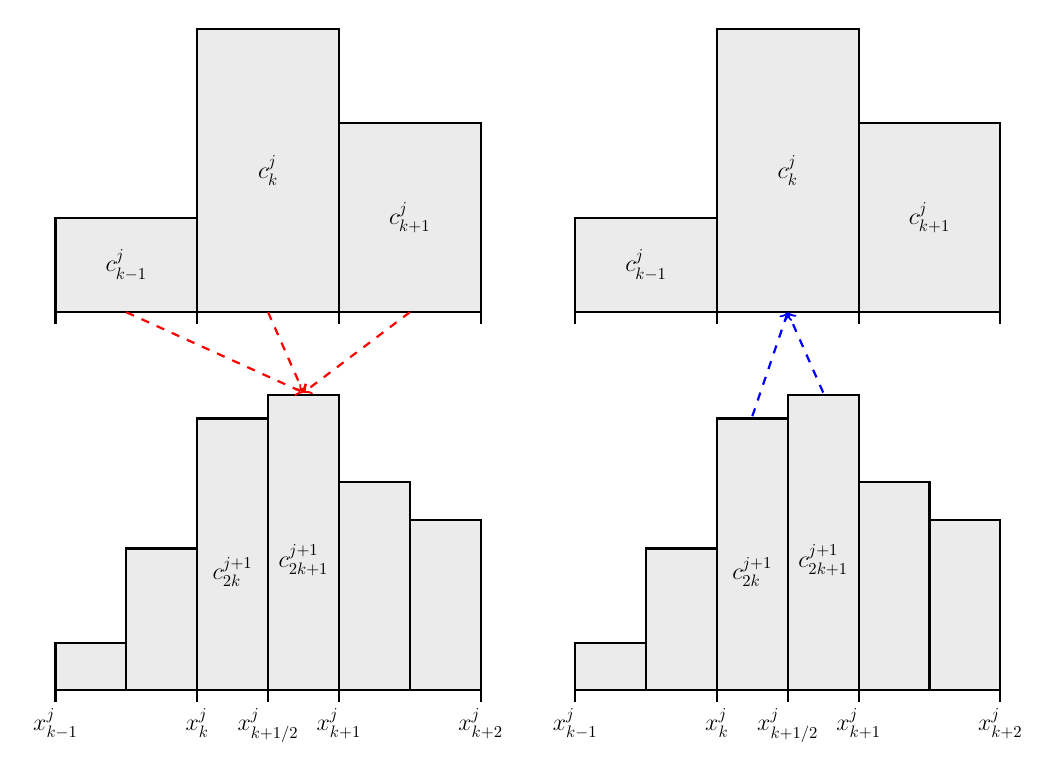
\begin{tikzpicture}[thick,scale=0.6, every node/.style={scale=0.6}]
    
        % variables
        \def\x{-8.0}
        \def\y{0.0}
        \def\yl{-8.0}
        
        % draw coarse level rectangles
        \draw [fill=mygray] (\x,0) rectangle (\x+3,2);
        \draw [fill=mygray] (\x+3,0) rectangle (\x+6,6);
        \draw [fill=mygray] (\x+6,0) rectangle (\x+9,4);
        
        % coarse level symbols
        \node at (\x+1.5,1) {\Large $c^{j}_{k-1}$};
        \node at (\x+4.5,3) {\Large $c^{j}_{k}$};
        \node at (\x+7.5,2) {\Large $c^{j}_{k+1}$};
        
        % coarse level axis
        \draw (\x,0) -- (\x,-0.25);
        \draw (\x+3,0) -- (\x+3,-0.25);
        \draw (\x+6,0) -- (\x+6,-0.25);
        \draw (\x+9,0) -- (\x+9,-0.25);

        % fine level rectangles
        \draw [fill=mygray] (\x,\yl) rectangle (\x+1.5,\yl+1);
        \draw [fill=mygray] (\x+1.5,\yl) rectangle (\x+3,\yl+3);
        \draw [fill=mygray] (\x+3,\yl) rectangle (\x+4.5,\yl+5.75);
        \draw [fill=mygray] (\x+4.5,\yl) rectangle (\x+6,\yl+6.25);
        \draw [fill=mygray] (\x+6,\yl) rectangle (\x+7.5,\yl+4.4);
        \draw [fill=mygray] (\x+7.5,\yl) rectangle (\x+9,\yl+3.6);
        
        % fine level symbols
        \node at (\x+3.75,\yl+2.5) {\Large $c^{j+1}_{2k}$};
        \node at (\x+5.25,\yl+2.75) {\Large $c^{j+1}_{2k+1}$};
        
        % fine level axis
	    \draw (\x,\yl) -- (\x,\yl-0.25);
        \draw (\x+3,\yl) -- (\x+3,\yl-0.25);
        \draw (\x+4.5,\yl) -- (\x+4.5,\yl-0.25);
        \draw (\x+6,\yl) -- (\x+6,\yl-0.25);
	    \draw (\x+9,\yl) -- (\x+9,\yl-0.25);

        % arrows
        \draw[red,dashed,->] (\x+1.5,\y) -- (\x+5.25,\y-1.7);
        \draw[red,dashed,->] (\x+4.5,\y) -- (\x+5.25,\y-1.7);
        \draw[red,dashed,->] (\x+7.5,\y) -- (\x+5.25,\y-1.7);

        % tick text
        \node[below] at (\x,\yl-0.25) {\Large $x^{j}_{k-1}$};
        \node[below] at (\x+3,\yl-0.25) {\Large $x^{j}_{k}$};
        \node[below] at (\x+4.5,\yl-0.25) {\Large $x^{j}_{k+1/2}$};
        \node[below] at (\x+6,\yl-0.25) {\Large $x^{j}_{k+1}$};
        \node[below] at (\x+9,\yl-0.25) {\Large $x^{j}_{k+2}$};
        
        %----
        
        % variables
        \def\x{3.0}
        \def\y{0.0}
        \def\yl{-8.0}
        
        % draw coarse level rectangles
        \draw [fill=mygray] (\x,0) rectangle (\x+3,2);
        \draw [fill=mygray] (\x+3,0) rectangle (\x+6,6);
        \draw [fill=mygray] (\x+6,0) rectangle (\x+9,4);
        
        % coarse level symbols
        \node at (\x+1.5,1) {\Large $c^{j}_{k-1}$};
        \node at (\x+4.5,3) {\Large $c^{j}_{k}$};
        \node at (\x+7.5,2) {\Large $c^{j}_{k+1}$};
        
        % coarse level axis
        \draw (\x,0) -- (\x,-0.25);
        \draw (\x+3,0) -- (\x+3,-0.25);
        \draw (\x+6,0) -- (\x+6,-0.25);
        \draw (\x+9,0) -- (\x+9,-0.25);

        % fine level rectangles
        \draw [fill=mygray] (\x,\yl) rectangle (\x+1.5,\yl+1);
        \draw [fill=mygray] (\x+1.5,\yl) rectangle (\x+3,\yl+3);
        \draw [fill=mygray] (\x+3,\yl) rectangle (\x+4.5,\yl+5.75);
        \draw [fill=mygray] (\x+4.5,\yl) rectangle (\x+6,\yl+6.25);
        \draw [fill=mygray] (\x+6,\yl) rectangle (\x+7.5,\yl+4.4);
        \draw [fill=mygray] (\x+7.5,\yl) rectangle (\x+9,\yl+3.6);
        
        % fine level symbols
        \node at (\x+3.75,\yl+2.5) {\Large $c^{j+1}_{2k}$};
        \node at (\x+5.25,\yl+2.75) {\Large $c^{j+1}_{2k+1}$};
        
        % fine level axis
	    \draw (\x,\yl) -- (\x,\yl-0.25);
        \draw (\x+3,\yl) -- (\x+3,\yl-0.25);
        \draw (\x+4.5,\yl) -- (\x+4.5,\yl-0.25);
        \draw (\x+6,\yl) -- (\x+6,\yl-0.25);
	    \draw (\x+9,\yl) -- (\x+9,\yl-0.25);

        % arrows
        \draw[blue,dashed,->] (\x+5.25,\y-1.7) -- (\x+4.5,\y);
        \draw[blue,dashed,->] (\x+3.75,\y-2.2) -- (\x+4.5,\y);

        % tick text
        \node[below] at (\x,\yl-0.25) {\Large $x^{j}_{k-1}$};
        \node[below] at (\x+3,\yl-0.25) {\Large $x^{j}_{k}$};
        \node[below] at (\x+4.5,\yl-0.25) {\Large $x^{j}_{k+1/2}$};
        \node[below] at (\x+6,\yl-0.25) {\Large $x^{j}_{k+1}$};
        \node[below] at (\x+9,\yl-0.25) {\Large $x^{j}_{k+2}$};
        

    \end{tikzpicture}
\end{figure}
\end{document}
